\chapter{Bio-anorganische chemie}\label{ch:b3:bioinorganic}

Ons bloed is rood door ijzer; het bloed van een degenkrab is kleurloos in
zijn aderen en wordt blauw aan de lucht, omdat het zuurstof op koper
vervoert. Het leven gebruikt een handvol metaalionen voor de taken die
geen enkele organische groep kan uitvoeren: zuurstof omkeerbaar binden,
afzonderlijke elektronen verplaatsen, water splitsen, stikstof
reduceren, een watermolecuul zuur genoeg maken om koolstofdioxide aan te
vallen. Dit hoofdstuk leest die taken met de instrumenten van de
coördinatiechemie: \omterm{def:b3:bioinorganic:hsab}{harde en zachte zuren}, ligandvelden en spintoestanden,
evenwichten en snelheidswetten, en het eindigt met de metalen die als
geneesmiddel gebruikt worden.

\begin{recall}
Het deel van jaar~2 behandelde $\alpha$-aminozuren, zijketens en peptiden, nucleobasen
en nucleotiden, coördinatiecomplexen, ligandvelden, hoogspin en laagspin,
en harde en zachte nucleofielen en elektrofielen; het deel van jaar~1
complexvormingsconstanten en de pL-schaal.
\Cref{ch:b3:complex-spectra-magnetism} en
\cref{ch:b3:complex-mechanisms} gaven spectra, de theorie van Marcus en
de aquatisering van cisplatine, \cref{ch:b3:complex-kinetics} de
kinetiek van Michaelis-Menten, en
\cref{ch:b3:advanced-nmr} de relaxatietijd $T_1$.
\end{recall}

\begin{omfigure}
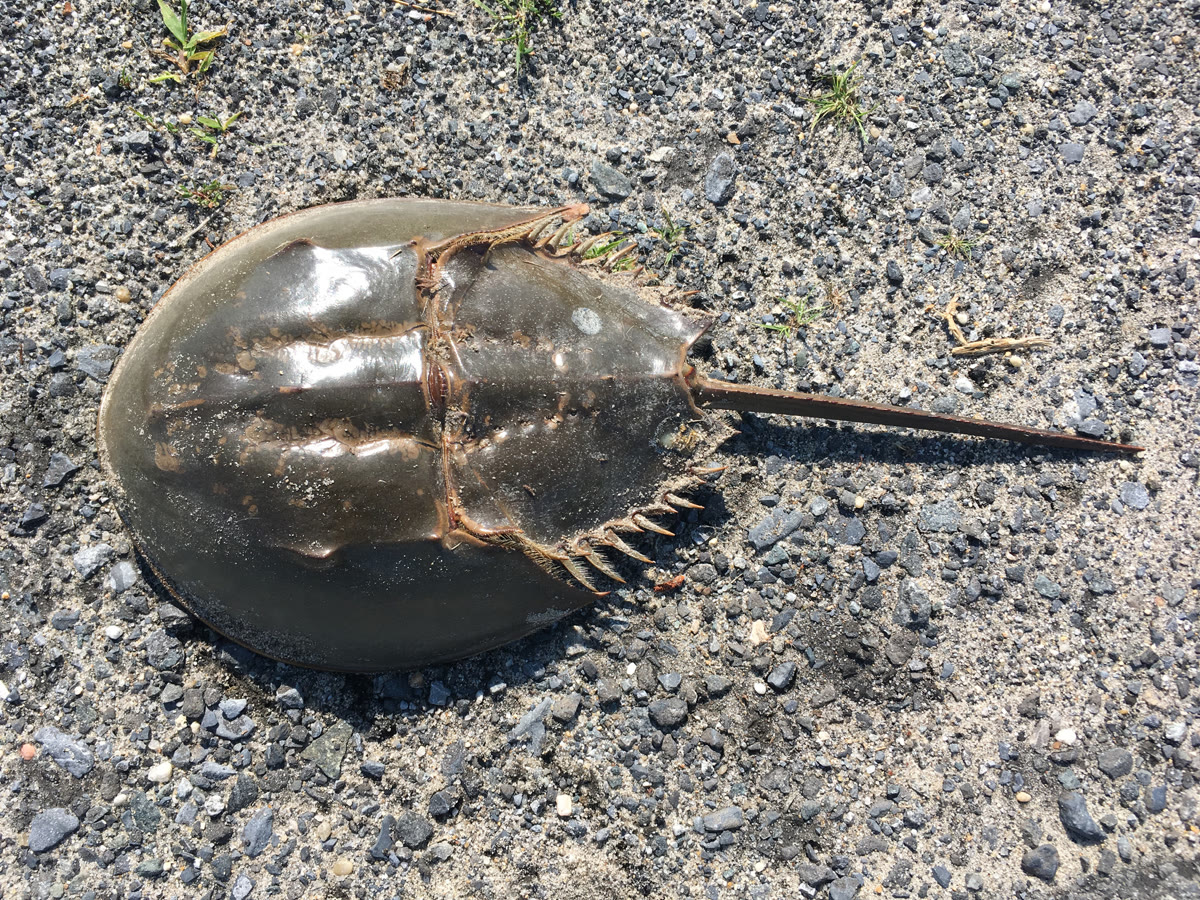
\includegraphics[width=0.5\linewidth]{images/book4/horseshoe-crab.jpg}

{\small Een Atlantische degenkrab. Zijn bloed vervoert zuurstof op
hemocyanine, een koperproteïne, en is blauw als het met zuurstof beladen
is. Foto: Kaldari, CC0.}
\end{omfigure}

\section{Metalen in de biologie}

\begin{definition}[Metalloproteïnen]\label{def:b3:bioinorganic:metalloprotein}
Een \emph{metalloproteïne}\index{metalloproteine@metalloproteïne} is een
eiwit dat gebonden metaalionen bevat; een
\emph{metallo-enzym}\index{metallo-enzym} is een metalloproteïne dat een
reactie katalyseert. Een \emph{cofactor}\index{cofactor} is een
niet-eiwitspecies, een metaalion of een klein molecuul, dat aan een eiwit
gebonden is en nodig is voor zijn activiteit.
\end{definition}

De metalen die in grote hoeveelheden tellen, zijn natrium, kalium,
magnesium en calcium, die vooral lading dragen en structuren
vasthouden; de overgangsmetalen ijzer, zink, koper, mangaan, kobalt,
molybdeen en nikkel komen in sporen voor, maar dragen een groot deel van
de chemie. Een eiwit kiest zijn metaal via de donoratomen die het aanbiedt
en hun geometrie.

\begin{definition}[Harde en zachte zuren]\label{def:b3:bioinorganic:hsab}
Een \emph{hard zuur}\index{hard zuur} is een klein, sterk geladen, weinig
polariseerbaar lewiszuur ($\ce{H+}$, $\ce{Mg^2+}$, $\ce{Ca^2+}$, $\ce{Fe^3+}$); een
\emph{zacht zuur}\index{zacht zuur} is een groot, polariseerbaar zuur met
een lage lading ($\ce{Cu+}$, $\ce{Ag+}$,
$\ce{Hg^2+}$, $\ce{Cd^2+}$). Het
\emph{principe van harde en zachte zuren en basen}\index{principe van harde en zachte zuren en basen}
stelt dat harde zuren bij voorkeur aan harde basen binden
(zuurstofdonoren, fluoride) en zachte zuren aan zachte basen
(zwaveldonoren, jodide).
\end{definition}

In eiwitten zijn carboxylaten en fenolaten hard, het thiolaat van
cysteïne en de thioether van methionine zacht, en het imidazool van
histidine zit ertussenin. IJzer(III) zit tussen zuurstofdonoren,
koper(I) tussen zwaveldonoren, zink, een grensgeval, bij histidine en
cysteïne; kwik en cadmium zijn onder meer giftig omdat ze de cysteïnes
van \omterm{def:b3:complex-kinetics:enzyme}{enzymen} inpikken.

\begin{definition}[Reeks van Irving-Williams]\label{def:b3:bioinorganic:irving-williams}
De \emph{reeks van Irving-Williams}\index{reeks van Irving-Williams} is de
volgorde van stabiliteit van de hoogspincomplexen van de tweewaardige
ionen van de eerste overgangsreeks met een gegeven ligand:
$\ce{Mn^2+} < \ce{Fe^2+} < \ce{Co^2+} < \ce{Ni^2+} < \ce{Cu^2+} > \ce{Zn^2+}$.
\end{definition}

\begin{proposition}[Volgorde van Irving-Williams]\label{prop:b3:bioinorganic:irving-williams}
De reeks geldt voor bijna alle liganden (een experimentele waarneming);
ze volgt de afname van de ionstraal van mangaan tot koper, de
ligandveldstabilisatie-energie, nul voor $d^5$, het grootst voor $d^8$, en de vervorming van
Jahn-Teller van koper(II), die vier van zijn bindingen verkort.
\end{proposition}

\begin{proof}[Beargumenteerd]
De straal neemt af over de rij naarmate de kernlading groeit, wat de
elektrostatische aantrekking van elk ligand versterkt. De
ligandveldstabilisatie van octaëdrische hoogspinionen
(\cref{ch:b3:complex-spectra-magnetism}) is $0$, $4$,
$8$, $12$ en $6\,\mathrm{Dq}$ voor $d^5$ tot $d^9$, en $0$ voor $d^{10}$: ze versterkt de trend tot nikkel en
valt weg voor zink; koper(II) wint meer terug dan zijn stabilisatie doet
vermoeden door zijn tetragonale vervorming, die vier korte, sterke
bindingen geeft.
\end{proof}

Een gevolg waarmee cellen moeten omgaan: koper en zink zouden de andere
ionen van de meeste plaatsen verdringen, zodat hun vrije concentraties
door gespecialiseerde transporteiwitten uiterst laag gehouden worden.

\section{Zuurstoftransport}

\begin{definition}[Porfyrinen en heem]\label{def:b3:bioinorganic:haem}
Een \emph{porfyrine}\index{porfyrine} is een grote, vlakke, aromatische
macrocyclus van vier pyrroolringen verbonden door methinebruggen, waarvan
de vier stikstofatomen een metaalion in het centrum binden.
\emph{Heem}\index{heem} is het ijzercomplex van protoporfyrine~IX, de
\omterm{def:b3:bioinorganic:metalloprotein}{cofactor} van hemoglobine, myoglobine en de cytochromen.
\end{definition}

In myoglobine en hemoglobine heeft het ijzer van het \omterm{def:b3:bioinorganic:haem}{heem} een vijfde
ligand onder de ring, het stikstofatoom van de proximale histidine, en een
zesde plaats die vrij is voor $\ce{O2}$.
Deoxy-ijzer(II) is hoogspin: een elektron in de $d_{x^2-y^2}$-orbitaal, die naar de vier
stikstofatomen wijst, maakt het te groot voor de opening van de ring, en
het zit buiten het vlak, naar de histidine toe. Bij het binden van $\ce{O2}$ wordt het laagspin, kleiner, en
schuift het in het vlak, waarbij het de histidine en de eiwithelix
meetrekt.

\begin{omfigure}
% ledger: pdb:Hb.deoxy.FeN4, pdb:Hb.oxy.FeN4
\begin{tikzpicture}[font=\small, scale=0.9]
  \foreach \x/\lab/\dz/\oxy in {0/deoxy (hoogspin)/-0.34/0, 6.4/oxy (laagspin)/-0.04/1} {
    \begin{scope}[xshift=\x cm]
      \draw[omDef, line width=2.6pt] (-2.2,0) -- (2.2,0);
      \node[font=\scriptsize, anchor=west, omDef] at (2.3,0) {porfyrine};
      \fill[omThm] (0,\dz*1.5) circle (0.22);
      \node[font=\scriptsize, anchor=north west] at (0.2,\dz*1.5-0.12) {Fe};
      \draw[black!70, line width=1pt] (0,\dz*1.5-0.22) -- (0,-1.55);
      \node[draw=black!70, regular polygon, regular polygon sides=5, minimum size=7mm, inner sep=0pt] at (0,-1.95) {};
      \node[font=\scriptsize, anchor=west] at (0.45,-1.95) {proximale His};
      \node[font=\small\bfseries] at (0,1.9) {\lab};
      \ifnum\oxy=1
        \draw[black!70, line width=1pt] (0,0.2) -- (0,0.85) -- (0.55,1.25);
        \fill[red!75] (0,0.85) circle (0.13) (0.55,1.25) circle (0.13);
        \node[font=\scriptsize, anchor=west] at (0.75,1.2) {$\ce{O2}$, gebogen};
      \fi
    \end{scope}
  }
  \draw[<->, black!60] (-1.0,0) -- (-1.0,-0.51) node[midway, left, font=\scriptsize] {\qty{0.34}{\angstrom}};
\end{tikzpicture}

{\small Het heemijzer van opzij gezien, met zijn verplaatsing ten opzichte
van de ring op schaal getekend (1~\AA{} als 1.35~cm; de andere afstanden zijn schematisch). In deoxyhemoglobine ligt het hoogspin-ijzer(II)
\qty{0.34}{\angstrom} onder het gemiddelde vlak van de vier pyrroolstikstofatomen, aan de kant van de
proximale histidine; in oxyhemoglobine ligt het binnen \qty{0.05}{\angstrom} van het vlak, met $\ce{O2}$
eindstandig en gebogen gebonden (afstanden berekend uit kristalstructuren).}
\end{omfigure}

Gebonden dizuurstof wordt beter beschreven als superoxide op ijzer(III), $\ce{Fe^{III}-O2^-}$, dan als
neutraal $\ce{O2}$ op ijzer(II): het complex is diamagnetisch omdat de ongepaarde
elektronen van de twee centra koppelen. Het eiwit verhindert de
onomkeerbare oxidatie tot ijzer(III) en water, die een vrij \omterm{def:b3:bioinorganic:haem}{heem} in water
onmiddellijk ondergaat.

\begin{definition}[Coöperatieve binding]\label{def:b3:bioinorganic:cooperativity}
Binding aan een eiwit met meerdere plaatsen is
\emph{coöperatief}\index{cooperatieve binding@coöperatieve binding}
als de binding van één ligand de affiniteit van de overige plaatsen
verhoogt. De \emph{hillcoëfficiënt}\index{hillcoefficient@hillcoëfficiënt} $n$ is de helling van de
hillgrafiek, $\log\frac{\theta}{1 - \theta}$ tegen $\log p$, bij halve verzadiging ($\theta$ is de fractie bezette
plaatsen).
\end{definition}

\begin{proposition}[Eén plaats]\label{prop:b3:bioinorganic:hyperbola}
Voor een eiwit met één plaats, $\mathrm{P + O_2 \rightleftharpoons PO_2}$, is de bezette fractie $\theta = p/(p_{50} + p)$, waarin $p_{50}$
de dissociatieconstante is, uitgedrukt als een druk.
\end{proposition}

\begin{proof}
$K_d = [\mathrm P]p/[\mathrm{PO_2}] = p_{50}$, dus $[\mathrm{PO_2}] = [\mathrm P]p/p_{50}$, en $\theta = [\mathrm{PO_2}]/([\mathrm P] + [\mathrm{PO_2}]) = (p/p_{50})/(1 + p/p_{50})$.
\end{proof}

\begin{theorem}[Vergelijking van Hill]\label{thm:b3:bioinorganic:hill}
Voor een eiwit met $n$ plaatsen die ofwel allemaal leeg ofwel allemaal bezet zijn,
$\mathrm{P + n\,O_2 \rightleftharpoons P(O_2)_n}$, is
\[
  \theta = \frac{p^n}{p_{50}^n + p^n}, \qquad \log\frac{\theta}{1 - \theta} = n\log p - n\log p_{50}.
\]
\end{theorem}

\begin{proof}
$K_d = [\mathrm P]p^n/[\mathrm{P(O_2)_n}]$; schrijf $K_d = p_{50}^n$. De fractie bezette plaatsen is die van de moleculen
in de bezette vorm, $\theta = [\mathrm{P(O_2)_n}]/([\mathrm P] + [\mathrm{P(O_2)_n}]) = (p/p_{50})^n/(1 + (p/p_{50})^n)$. Dan is $\theta/(1 - \theta) = (p/p_{50})^n$, en de
logaritme nemen geeft de rechte met helling $n$.
\end{proof}

Hemoglobine, met vier plaatsen, is niet volledig \omterm{def:b3:bioinorganic:cooperativity}{coöperatief}: zijn
\omterm{def:b3:bioinorganic:cooperativity}{hillcoëfficiënt} ligt ruim onder 4, rond 3, en zijn hillgrafiek heeft
helling 1 aan beide uiteinden, waar het zich gedraagt als een deoxy- of
een oxyeiwit met onafhankelijke plaatsen. De coöperativiteit komt van een
verandering van de quaternaire structuur: de verschuiving van het ijzer
in het vlak van het eerste \omterm{def:b3:bioinorganic:haem}{heem} dat $\ce{O2}$ bindt, wordt doorgegeven aan de andere subeenheden.

\begin{omfigure}
\begin{tikzpicture}
\begin{axis}[name=a, width=0.48\linewidth, height=5.6cm, xmin=0, xmax=14, ymin=0, ymax=1.02,
  axis lines=left, xlabel={$p(\ce{O2})$ / \unit{kPa}}, ylabel={verzadiging $\theta$},
  tick label style={font=\scriptsize}, label style={font=\small}]
\addplot[omMeth, thick] table[x=p, y=Mb] {figdata/out/bachelor-3-oxygen-binding.dat};
\addplot[omThm, thick] table[x=p, y=Hb] {figdata/out/bachelor-3-oxygen-binding.dat};
\addplot[omThm, thick, dashed] table[x=p, y=Hbacid] {figdata/out/bachelor-3-oxygen-binding.dat};
\draw[black!35] (axis cs:5,0) -- (axis cs:5,1.0) (axis cs:13,0) -- (axis cs:13,1.0);
\node[font=\scriptsize, anchor=south] at (axis cs:5,0.02) {weefsels};
\node[font=\scriptsize, anchor=south east] at (axis cs:13,0.02) {longen};
\node[font=\scriptsize, omMeth] at (axis cs:1.9,0.96) {Mb};
\node[font=\scriptsize, omThm] at (axis cs:7.5,0.6) {Hb};
\end{axis}
\begin{axis}[at={(a.east)}, anchor=west, xshift=1.4cm, width=0.48\linewidth, height=5.6cm,
  xmin=-1.5, xmax=1.5, ymin=-3, ymax=3, axis lines=left,
  xlabel={$\log_{10}(p/\unit{kPa})$}, ylabel={$\log_{10}\bigl(\theta/(1-\theta)\bigr)$},
  tick label style={font=\scriptsize}, label style={font=\small}]
\draw[black!30] (axis cs:-1.5,0) -- (axis cs:1.5,0);
\addplot[omMeth, thick] table[x=lgp, y=Mb] {figdata/out/bachelor-3-oxygen-binding-b.dat};
\addplot[omThm, thick, restrict y to domain=-3:3] table[x=lgp, y=Hb] {figdata/out/bachelor-3-oxygen-binding-b.dat};
\node[font=\scriptsize, omMeth, anchor=west] at (axis cs:-1.1,1.4) {helling 1};
\node[font=\scriptsize, omThm, anchor=west] at (axis cs:0.75,-1.5) {helling 2.7};
\end{axis}
\end{tikzpicture}

{\small Links: zuurstofverzadiging van myoglobine (groen) en hemoglobine
(rood; gestreept: bij een lagere pH) tegen de zuurstofdruk, met de
modelwaarden
$p_{50} = \qty{0.37}{kPa}$ (Mb) en \qty{3.5}{kPa} (Hb), $n = 2.7$. Tussen de longen en de weefsels staat
hemoglobine een kwart van zijn zuurstof af, myoglobine bijna niets.
Rechts: de overeenkomstige hillgrafieken, rechten in dit model (de
grafiek van echt hemoglobine buigt aan beide uiteinden af naar helling
1).}
\end{omfigure}

\begin{method}[Een hillgrafiek aflezen]\label{met:b3:bioinorganic:hill-plot}
\begin{enumerate}
  \item Bereken uit elke gemeten verzadiging $\log(\theta/(1 - \theta))$; zet het uit tegen $\log p$.
  \item De druk waarbij de grafiek nul snijdt, is $p_{50}$.
  \item De helling in dat punt is de \omterm{def:b3:bioinorganic:cooperativity}{hillcoëfficiënt}: $n = 1$ betekent onafhankelijke
        plaatsen, $n > 1$ \omterm{def:b3:bioinorganic:cooperativity}{coöperatieve binding}.
  \item Met slechts twee punten is $n = \Delta\log(\theta/(1 - \theta))/\Delta\log p$.
\end{enumerate}
\end{method}

Hemoglobine bindt ook protonen en koolstofdioxide op plaatsen buiten het
\omterm{def:b3:bioinorganic:haem}{heem}, die zijn kromme naar rechts verschuiven waar ze overvloedig zijn,
in werkende weefsels: het bohreffect zet meer zuurstof vrij precies daar
waar ze nodig is.

\begin{proposition}[Competitie met koolstofmonoxide]\label{prop:b3:bioinorganic:haldane}
Als koolstofmonoxide en dizuurstof om dezelfde plaatsen concurreren, met
$\mathrm{HbO_2 + CO \rightleftharpoons HbCO + O_2}$ met evenwichtsconstante $M$, dan is
$[\mathrm{HbCO}]/[\mathrm{HbO_2}] = M\,p(\ce{CO})/p(\ce{O2})$.
\end{proposition}

\begin{proof}
In evenwicht is $M = [\mathrm{HbCO}]\,p(\ce{O2})/([\mathrm{HbO_2}]\,p(\ce{CO}))$; herschikken geeft het resultaat.
\end{proof}

$M$ ligt in de honderden voor menselijk hemoglobine, zodat enkele honderden
ppm koolstofmonoxide een groot deel van de plaatsen bezetten; erger nog,
de plaatsen die vrij blijven, houden hun zuurstof steviger vast, omdat de
coöperativiteit op hen inwerkt. Vrij \omterm{def:b3:bioinorganic:haem}{heem} bindt koolstofmonoxide nog
veel sterker: in het eiwit hindert een distale histidine boven het ijzer
de lineaire geometrie Fe--C--O
die koolstofmonoxide verkiest, terwijl ze een waterstofbrug vormt met het gebogen $\ce{O2}$.
Andere dieren gebruiken andere metalen: de hemocyaninen van weekdieren
en geleedpotigen binden $\ce{O2}$ als peroxide tussen twee koperionen, de hemerytrinen van sommige
zeewormen op een paar ijzerionen.

\begin{inthelab}[Een zuurstofbindingscurve]
Een oplossing van hemoglobine in buffer wordt in een gasdichte cuvet met
een zijkolf gebracht. Ze wordt eerst van zuurstof ontdaan door spoelen
met stikstof, daarna worden bekende volumes lucht ingespoten en wordt de
oplossing door zacht kantelen in evenwicht gebracht. Na elke toevoeging
wordt het zichtbare spectrum opgenomen: de banden van de deoxyvorm (één
band rond \qty{555}{nm}) maken plaats voor de twee banden van de oxyvorm,
en de verzadiging wordt afgelezen uit de absorbantie bij één golflengte,
tussen haar deoxy- en oxylimiet.
\end{inthelab}

\section{Metallo-enzymen}

Koolzuuranhydrase versnelt $\ce{CO2 + H2O <=> HCO3- + H+}$, dat in water alleen seconden
duurt, wat genoeg is om ertoe te doen tijdens de korte doortocht van een
rode bloedcel door een longcapillair. Zijn zinkion wordt vastgehouden
door drie histidines en een watermolecuul. Als klein kation met een hoge
lading verlaagt het de $\mathrm pK_a$ van dat water van ongeveer 14 tot
ongeveer 7: bij fysiologische pH draagt een groot deel van het \omterm{def:b3:complex-kinetics:enzyme}{enzym} een
aan zink gebonden hydroxide, een sterk nucleofiel, vlak naast een holte
die $\ce{CO2}$ bindt.

\begin{omfigure}
\begin{tikzpicture}[font=\small, >=Stealth]
  \node (a) at (90:2.0) {$\mathrm{(His)_3Zn{-}OH_2}$};
  \node (b) at (0:2.9) {$\mathrm{(His)_3Zn{-}OH^-}$};
  \node (c) at (-90:2.0) {$\mathrm{(His)_3Zn{-}OCO_2H^-}$};
  \draw[->, thick] (a) to[bend left=25] node[midway, above right, font=\scriptsize] {$-\,\ce{H+}$ (naar een histidinependel)} (b);
  \draw[->, thick] (b) to[bend left=25] node[midway, below right, font=\scriptsize, align=left] {$+\,\ce{CO2}$:\\ nucleofiele aanval} (c);
  \draw[->, thick] (c) to[bend left=35] node[midway, left, font=\scriptsize, align=right] {$+\,\ce{H2O}$\\ $-\,\ce{HCO3-}$} (a);
\end{tikzpicture}

{\small De katalytische cyclus van koolzuuranhydrase. Het aan zink
gebonden water verliest een proton; het aan zink gebonden hydroxide valt
koolstofdioxide aan; water verdringt het waterstofcarbonaat. De
protonoverdracht naar het oplosmiddel is de traagste stap.}
\end{omfigure}

\begin{proposition}[Een snel enzym]\label{prop:b3:bioinorganic:carbonic-anhydrase}
De \omterm{def:b3:complex-kinetics:michaelis}{specificiteitsconstante} $k_{\mathrm{cat}}/K_M$ van koolzuuranhydrase nadert de
snelheidsconstante van de ontmoeting van $\ce{CO2}$ met het \omterm{def:b3:complex-kinetics:enzyme}{enzym}: bijna elke ontmoeting leidt tot
reactie.
\end{proposition}

\begin{proof}[Beargumenteerd]
$k_{\mathrm{cat}}/K_M$ is de tweedeordesnelheidsconstante van \omterm{def:b3:complex-kinetics:enzyme}{enzym} en substraat bij lage
substraatconcentratie (\cref{ch:b3:complex-kinetics}); ze kan niet groter
zijn dan de snelheidsconstante van hun diffusiegecontroleerde ontmoeting
(\cref{ch:b3:rate-theories}). De gemeten waarden voor koolzuuranhydrase
behoren tot de hoogste die van enig \omterm{def:b3:complex-kinetics:enzyme}{enzym} bekend zijn en naderen die
limiet: de chemie in de \omterm{def:b3:complex-kinetics:enzyme}{actieve plaats} is dan niet langer wat de snelheid
beperkt.
\end{proof}

Cytochroom-P450-enzymen, in de lever en in veel andere cellen,
hydroxyleren bindingen C--H van geneesmiddelen en hormonen. Hun heemijzer wordt vastgehouden door een
cysteïnethiolaat; met
$\ce{O2}$ en twee elektronen vormt het een ijzer(IV)-oxocomplex met een radicaal op de
\omterm{def:b3:bioinorganic:haem}{porfyrine}, compound I genoemd, dat een waterstofatoom aan het substraat
onttrekt en de hydroxylgroep teruggeeft aan het koolstofradicaal.
Nitrogenase reduceert $\ce{N2}$ tot ammoniak bij kamertemperatuur op een cluster van zeven ijzeratomen,
één molybdeenatoom en negen sulfiden rond een centraal koolstofatoom, de
\omterm{def:b3:bioinorganic:metalloprotein}{FeMo-cofactor}, ten koste van veel moleculen ATP. Vitamine $\mathrm{B_{12}}$ bevat een
kobalt-koolstofbinding, een van de zeer weinige metaal-koolstofbindingen
in de biologie, waarvan de homolyse radicaalomleggingen op gang brengt.

\section{Elektronenoverdracht en energie}

Eiwitten die alleen elektronen verplaatsen, hebben metaalcentra met
kleine reorganisatie-energieën (\cref{ch:b3:complex-mechanisms}): de twee
oxidatietoestanden hebben bijna dezelfde geometrie, zodat de barrière van
Marcus laag is.

\begin{definition}[IJzer-zwavelclusters]\label{def:b3:bioinorganic:fes}
Een \emph{ijzer-zwavelcluster}\index{ijzer-zwavelcluster} is een groep
ijzerionen die overbrugd worden door sulfide-ionen en via
cysteïnethiolaten aan het eiwit gebonden zijn:
$\ce{[2Fe-2S]}$, $\ce{[3Fe-4S]}$ en het kubaanachtige $\ce{[4Fe-4S]}$.
\end{definition}

\begin{definition}[Blauwe koperproteïnen]\label{def:b3:bioinorganic:blue-copper}
Een \emph{blauwe koperproteïne}\index{blauwe koperproteine@blauwe koperproteïne}
draagt één koperion, gebonden door twee histidines, een cysteïne en een
zwak gebonden methionine in een vervormde tetraëdrische plaats; haar
intense blauwe kleur komt van een ladingsoverdrachtsband van cysteïne
naar koper(II).
\end{definition}

\begin{definition}[Entatische toestand]\label{def:b3:bioinorganic:entatic}
De \emph{entatische toestand}\index{entatische toestand} is een
metaalplaats die door het eiwit in een gespannen geometrie gehouden
wordt, tussen de geometrieën die zijn twee oxidatietoestanden verkiezen,
wat de \omterm{def:b3:complex-mechanisms:reorganisation}{reorganisatie-energie} van zijn reacties verlaagt.
\end{definition}

Koper(II) alleen verkiest een vierkant vlak, koper(I) een tetraëder: in de
plaats van de \omterm{def:b3:bioinorganic:blue-copper}{blauwe koperproteïnen} is geen van beide tevreden, en de
elektronenoverdracht is snel.

\begin{definition}[Zuurstofontwikkelend complex]\label{def:b3:bioinorganic:oec}
Het \emph{zuurstofontwikkelend complex}\index{zuurstofontwikkelend complex}
van fotosysteem~II is de cluster $\mathrm{Mn_4CaO_5}$ die water bij de fotosynthese oxideert tot
dizuurstof.
\end{definition}

\begin{proposition}[Vier fotonen per zuurstofmolecuul]\label{prop:b3:bioinorganic:kok}
De oxidatie van twee watermoleculen tot één $\ce{O2}$ vereist vier fotonen
die door fotosysteem~II geabsorbeerd worden, waarbij de cluster vijf toestanden $\mathrm S_0$ tot $\mathrm S_4$ doorloopt.
\end{proposition}

\begin{proof}
$\ce{2H2O -> O2 + 4H+ + 4e-}$: er moeten vier elektronen weggenomen worden. Elk foton dat door het
reactiecentrum geabsorbeerd wordt, verplaatst één elektron weg van dat
centrum, en de cluster vult het geoxideerde centrum elektron per
elektron weer aan: vier fotonen, vier stappen, waarbij oxiderende
equivalenten opgeslagen worden in de toestanden $\mathrm S_1$ tot $\mathrm S_4$; $\mathrm S_4$ zet $\ce{O2}$ vrij en keert terug naar $\mathrm S_0$.
\end{proof}

\begin{omfigure}
\begin{tikzpicture}[font=\small, >=Stealth]
  \foreach \i/\ang in {0/90, 1/18, 2/-54, 3/-126, 4/162} {
    \node[draw, circle, minimum size=9mm, fill=omDef!10] (s\i) at (\ang:2.0) {$\mathrm S_{\i}$};
  }
  \foreach \i/\j in {0/1, 1/2, 2/3, 3/4} {
    \draw[->, thick] (s\i) to[bend left=18] node[midway, sloped, above, font=\scriptsize] {$h\nu$, $-\mathrm e^-$} (s\j);
  }
  \draw[->, thick, omThm] (s4) to[bend left=18] node[midway, sloped, above, font=\scriptsize] {$-\ce{O2}$, $+\,\ce{2H2O}$} (s0);
\end{tikzpicture}

{\small De kokcyclus van het \omterm{def:b3:bioinorganic:oec}{zuurstofontwikkelend complex}. Elk foton dat
door fotosysteem~II geabsorbeerd wordt, neemt één elektron weg van de
mangaancluster (onderweg vertrekken protonen); de vierde oxidatie geeft $\mathrm S_4$, dat dizuurstof vrijzet en
opnieuw twee watermoleculen bindt.}
\end{omfigure}

Aan het andere uiteinde van de energieketen reduceert het
cytochroom-$c$-oxidase van de
mitochondriën $\ce{O2}$ tot water met vier elektronen en vier protonen op een
heemijzer en een koperion die tegenover elkaar staan, zonder het
gedeeltelijk gereduceerde, schadelijke superoxide of peroxide vrij te
laten.

\section{Metalen in de geneeskunde}

\begin{definition}[Metallogeneesmiddelen]\label{def:b3:bioinorganic:metallodrug}
Een \emph{metallogeneesmiddel}\index{metallogeneesmiddel} is een
geneesmiddel waarvan de werking afhangt van een metaalion of een
metaalcomplex.
\end{definition}

Cisplatine, \textit{cis}-$\ce{[PtCl2(NH3)2]}$, is stabiel in het bloed, waar de chlorideconcentratie
hoog is; in cellen, waar ze veel lager is, wisselt het een chloride uit
tegen water (\cref{ch:b3:complex-mechanisms}). Het aquacomplex bindt het
atoom N7 van guanine, daarna een tweede guanine ernaast op dezelfde
streng: de 1,2-GG-kruisbinding buigt het DNA, dat de cel niet kan
herstellen, en de cel sterft. Het isomeer
\textit{trans} kan geen twee naburige basen overbruggen en is inactief.
Carboplatine, met een chelerend dicarboxylaat dat traag vertrekt, heeft
minder bijwerkingen; oxaliplatine, met een diaminocyclohexaanligand,
werkt op tumoren die resistent zijn tegen cisplatine.

\begin{omfigure}
\begin{tikzpicture}[font=\small]
  \draw[black!60, line width=1.4pt] (-3.2,0) -- (3.2,0);
  \node[font=\scriptsize, anchor=west] at (3.3,0) {DNA-streng};
  \foreach \x/\b in {-2.4/C, -1.0/G, 1.0/G, 2.4/T} {
    \draw[black!60, line width=1pt] (\x,0) -- (\x,0.6);
    \node[draw=black!70, fill=white, rounded corners=1pt, minimum width=6mm] (n\b\x) at (\x,0.9) {\b};
  }
  \node (pt) at (0,2.4) {$\ce{Pt}$};
  \draw[omThm, thick] (pt) -- (-0.95,1.2) node[midway, left, font=\scriptsize] {N7};
  \draw[omThm, thick] (pt) -- (0.95,1.2) node[midway, right, font=\scriptsize] {N7};
  \draw (pt) -- (-0.5,3.1) node[above left, font=\scriptsize, inner sep=1pt] {$\ce{H3N}$};
  \draw (pt) -- (0.5,3.1) node[above right, font=\scriptsize, inner sep=1pt] {$\ce{NH3}$};
\end{tikzpicture}

{\small De 1,2-kruisbinding binnen één streng die cisplatine maakt,
schematisch: na het verlies van zijn twee chloriden bindt platina de
atomen N7 van twee naburige guanines van één streng, en behoudt het zijn
twee \textit{cis}-ammineliganden. Het echte adduct buigt de dubbele helix.}
\end{omfigure}

\begin{definition}[Contrastmiddelen]\label{def:b3:bioinorganic:contrast}
Een \emph{contrastmiddel}\index{contrastmiddel} voor
magnetische-resonantiebeeldvorming is een paramagnetische verbinding die
de relaxatietijden van nabije waterprotonen verkort. Zijn
\emph{relaxiviteit}\index{relaxiviteit} $r_1$ is de toename van de
relaxatiesnelheid $1/T_1$ per eenheid van concentratie van het middel.
\end{definition}

\begin{proposition}[Relaxatiesnelheid]\label{prop:b3:bioinorganic:relaxivity}
Met een middel met \omterm{def:b3:bioinorganic:contrast}{relaxiviteit} $r_1$ bij concentratie $c$ is de relaxatiesnelheid van de
waterprotonen $1/T_1 = 1/T_{1,0} + r_1c$, waarin $T_{1,0}$ de waarde zonder middel is.
\end{proposition}

\begin{proof}
De paramagnetische bijdrage is evenredig met het aantal moleculen van
het middel dat watermoleculen per tijdseenheid bezoeken, dus met $c$;
relaxatiesnelheden van onafhankelijke mechanismen tellen op. Volgens de definitie van $r_1$ is de toegevoegde snelheid $r_1c$.
\end{proof}

Gadolinium(III), $4f^7$ met zeven ongepaarde elektronen en een traag
relaxerende elektronenspin, is het metaal bij uitstek. Vrij $\ce{Gd^3+}$ is giftig: het wordt toegediend als een
zeer stabiel complex van een achttandig polyaminocarboxylaat dat één
plaats vrijlaat voor een watermolecuul, dat snel met het vrije water
uitwisselt en de relaxatie naar het hele water overbrengt.

\begin{definition}[Chelatietherapie]\label{def:b3:bioinorganic:chelation-therapy}
\emph{Chelatietherapie}\index{chelatietherapie} is het verwijderen van een
giftig metaal uit het lichaam met een chelerend ligand dat als
geneesmiddel toegediend wordt en een stabiel, oplosbaar complex vormt dat
uitgescheiden wordt.
\end{definition}

\begin{method}[Een chelerend geneesmiddel kiezen]\label{met:b3:bioinorganic:choose-chelator}
\begin{enumerate}
  \item Vergelijk de stabiliteitsconstanten van de chelator met het giftige
        metaal en met de essentiële metalen die in grote hoeveelheden
        aanwezig zijn ($\ce{Ca^2+}$, $\ce{Mg^2+}$,
        $\ce{Zn^2+}$).
  \item Bereken het vrije metaalniveau $\mathrm{pM} = -\log[\mathrm M]$ dat de chelator overlaat bij de
        concentraties en de pH van het lichaam: hoe hoger pM voor het
        giftige metaal en hoe lager voor de essentiële, hoe beter.
  \item Dien de chelator al beladen met het concurrerende essentiële ion
        toe (het calciumcomplex van EDTA voor lood), zodat hij uitwisselt
        in plaats van calcium aan het bloed te onttrekken.
  \item Controleer de hard-zachtovereenkomst (zwaveldonoren voor kwik en
        lood, harde zuurstofdonoren voor ijzer(III)) en of het complex
        uitgescheiden wordt.
\end{enumerate}
\end{method}

\begin{safety}{\ghs[0.62cm]{GHS05}\ghs[0.62cm]{GHS06}\ghs[0.62cm]{GHS08}}
% ledger: ghs4:cisplatin
Cisplatine: dodelijk bij inslikken, kan kanker en genetische defecten
veroorzaken, kan de vruchtbaarheid schaden, veroorzaakt ernstig
oogletsel en allergische reacties; het wordt alleen gehanteerd als
bereide geneesmiddeloplossing, met handschoenen, in een geventileerde
kast.
\end{safety}

\begin{history}[Een eiwitstructuur en een toevallig geneesmiddel]
Max Perutz werkte meer dan twintig jaar aan de röntgenstructuur van
hemoglobine, die in 1959 bij lage resolutie opgelost werd; met John
Kendrew, die myoglobine oploste, ontving hij de Nobelprijs voor de
Scheikunde van 1962. In 1965 zag Barnett Rosenberg, die een stroom
tussen platina-elektroden door een bacteriecultuur stuurde, de bacteriën
uitgroeien tot lange draden zonder te delen; de oorzaak was niet de
stroom, maar een platina-amminecomplex dat uit de elektroden gevormd
werd. Het werd cisplatine, nog steeds een van de meest gebruikte
antikankermiddelen.
\end{history}

\section{Oefeningen}

\begin{exercise}[$\star$]\label{exo:b3:bioinorganic:1}
Een eiwit is voor 20\,\% verzadigd bij \qty{2.1}{kPa} zuurstof en voor 80\,\% bij \qty{5.9}{kPa}. Bereken zijn
\omterm{def:b3:bioinorganic:cooperativity}{hillcoëfficiënt}.
\end{exercise}

\begin{exercise}[$\star$]\label{exo:b3:bioinorganic:2}
Rangschik $\ce{Zn^2+}$, $\ce{Mn^2+}$, $\ce{Cu^2+}$, $\ce{Fe^2+}$, $\ce{Ni^2+}$ en $\ce{Co^2+}$ naar de stabiliteit van hun complexen met
een gegeven ligand, en verklaar de plaats van zink.
\end{exercise}

\begin{exercise}[$\star$]\label{exo:b3:bioinorganic:3}
Voorspel de donoren van eiwitten (carboxylaat, cysteïnethiolaat,
histidine-imidazool) waaraan $\ce{Ca^2+}$, $\ce{Fe^3+}$, $\ce{Cu+}$, $\ce{Zn^2+}$ en $\ce{Hg^2+}$ de voorkeur geven.
\end{exercise}

\begin{exercise}[$\star$]\label{exo:b3:bioinorganic:4}
Hoeveel elektronen worden er weggenomen, en hoeveel fotonen door
fotosysteem~II geabsorbeerd,
per ontwikkeld molecuul $\ce{O2}$? Per mol?
\end{exercise}

\begin{exercise}[$\star\star$]\label{exo:b3:bioinorganic:5}
Bereken met de modelkrommen van het hoofdstuk ($p_{50} = \qty{0.37}{kPa}$ voor myoglobine; \qty{3.5}{kPa} en $n = 2.7$ voor
hemoglobine) welke fractie van zijn zuurstof elk eiwit afstaat tussen
\qty{13}{kPa} (longen) en \qty{5}{kPa} (weefsels).
\end{exercise}

\begin{exercise}[$\star\star$]\label{exo:b3:bioinorganic:6}
Lucht met \qty{50}{ppm} koolstofmonoxide wordt lang genoeg ingeademd om
het evenwicht te bereiken. Welke fractie van het hemoglobine draagt CO,
met $M = 230$ (gegevens van de oefening) en $p(\ce{O2})/p(\ce{CO})$ zoals in de lucht
(20.95\,\% zuurstof)?
\end{exercise}

\begin{exercise}[$\star\star$]\label{exo:b3:bioinorganic:7}
Geef de formele oxidatietoestanden van de ijzerionen in de clusters $\ce{[Fe2S2(SR)4]^2-}$,
$\ce{[Fe2S2(SR)4]^3-}$ en $\ce{[Fe4S4(SR)4]^2-}$ (SR: cysteïnaat, S: sulfide).
\end{exercise}

\begin{exercise}[$\star\star$]\label{exo:b3:bioinorganic:8}
Schrijf de eerste aquatisering van cisplatine op, en leg uit waarom ze
traag verloopt in het bloed en sneller in cellen. Aan welk atoom van het
DNA bindt platina, en waarom is het isomeer
\textit{trans} inactief?
\end{exercise}

\begin{exercise}[$\star\star$]\label{exo:b3:bioinorganic:9}
Een weefsel heeft $T_1 = \qty{1.2}{s}$. Een gadoliniummiddel met \omterm{def:b3:bioinorganic:contrast}{relaxiviteit} $\qty{4.0}{L.mmol^{-1}.s^{-1}}$ bereikt er \qty{0.10}{mmol/L}
(gegevens van de oefening). Bereken de nieuwe $T_1$.
\end{exercise}

\begin{exercise}[$\star\star\star$]\label{exo:b3:bioinorganic:10}
Een chelator L heeft $\log K = 18.0$ met $\ce{Pb^2+}$ en $10.7$ met $\ce{Ca^2+}$ (gegevens van de oefening).
Bereken de evenwichtsconstante van $\ce{Pb^2+ + [CaL]^2- <=> [PbL]^2- + Ca^2+}$ en leg uit waarom men het
calciumcomplex toedient en niet het vrije ligand.
\end{exercise}

\begin{exercise}[$\star\star\star$]\label{exo:b3:bioinorganic:11}
% ledger: enz:median.kcatKM
Koolzuuranhydrase heeft $k_{\mathrm{cat}}/K_M \approx \qty{1e8}{L.mol^{-1}.s^{-1}}$ (gegevens van de oefening), een typisch \omterm{def:b3:complex-kinetics:enzyme}{enzym} ongeveer
$\qty{1e5}{L.mol^{-1}.s^{-1}}$. Vergelijk bij $[\ce{CO2}] = \qty{1.0}{mmol/L}$, ver onder $K_M$, de tijd die elk nodig heeft om de helft
van het substraat om te zetten bij een enzymconcentratie van \qty{1.0}{\micro mol/L}.
\end{exercise}

\begin{exercise}[$\star\star\star$]\label{exo:b3:bioinorganic:12}
Welke druk koolstofmonoxide bezet met $M = 230$ de helft van de plaatsen
in aanwezigheid van lucht met \qty{0.2095}{bar} zuurstof? Druk haar uit in ppm van een gas bij \qty{1}{bar}.
\end{exercise}

\section{Probleem: hoeveel zuurstof levert het bloed?}

\begin{problem}[{Weekendprobleem --- hoeveel zuurstof levert het bloed?
Hillkrommen van hemoglobine en myoglobine, de zuurstof die een liter
bloed vervoert, de bohrverschuiving, en wat koolstofmonoxide wegneemt}]
\label{pb:b3:bioinorganic:1}
% ledger: const:Vm1
Modelgegevens van het probleem: hemoglobine $p_{50} = \qty{3.5}{kPa}$ en $n = 2.7$ bij pH 7.4, $p_{50} = \qty{4.0}{kPa}$ bij de
lagere pH van werkende weefsels; myoglobine $p_{50} = \qty{0.37}{kPa}$; bloed bevat \qty{150}{g/L}
hemoglobine, met molaire massa \qty{64.5}{kg/mol} en vier plaatsen per molecuul; $p(\ce{O2})$ is \qty{13}{kPa}
in de longen en \qty{5.0}{kPa} in de weefsels; het hart pompt in rust \qty{5.0}{L/min};
$M = 230$ voor koolstofmonoxide. Gasvolumes bij \qty{273.15}{K} en \qty{101.325}{kPa}.

\medskip\noindent\textbf{Deel I --- De krommen.}
\begin{enumerate}
  \item Bereken de verzadiging van hemoglobine in de longen.
  \item Bereken haar in de weefsels bij pH 7.4.
  \item Bereken de verzadiging van myoglobine bij \qty{5.0}{kPa}.
  \item Waarom kan myoglobine in een spier zuurstof van hemoglobine
        overnemen?
  \item Welke \omterm{def:b3:bioinorganic:cooperativity}{hillcoëfficiënt} zouden vier onafhankelijke plaatsen geven?
  \item Leg in één zin uit waar de coöperativiteit vandaan komt.
\end{enumerate}

\medskip\noindent\textbf{Deel II --- Een liter bloed.}
\begin{enumerate}[resume]
  \item Bereken de concentratie hemoglobine in mol/L.
  \item Bereken de concentratie zuurstofplaatsen.
  \item Bereken de zuurstof die per liter in de longen vervoerd wordt, in
        mmol.
  \item Bereken de zuurstof die per liter bij pH 7.4 aan de weefsels
        geleverd wordt.
  \item Reken die om naar milliliter gas.
  \item Welke fractie van de vervoerde zuurstof is dat?
\end{enumerate}

\medskip\noindent\textbf{Deel III --- De bohrverschuiving.}
\begin{enumerate}[resume]
  \item Bereken de verzadiging in de weefsels bij de lagere pH.
  \item Bereken de zuurstof die met de verschuiving per liter geleverd
        wordt.
  \item Met welke factor verhoogt de verschuiving de levering?
  \item Wat verlaagt de pH van een werkende spier?
  \item Bereken de zuurstof die per minuut in rust geleverd wordt, in
        mmol.
  \item Reken die om naar liter gas per minuut.
\end{enumerate}

\medskip\noindent\textbf{Deel IV --- Koolstofmonoxide.}
\begin{enumerate}[resume]
  \item Bereken $[\mathrm{HbCO}]/[\mathrm{HbO_2}]$ voor lucht met \qty{100}{ppm} CO.
  \item Bereken de fractie plaatsen die aan CO verloren gaat.
  \item Waarom is het verlies aan geleverde zuurstof groter dan die
        fractie?
  \item Waarom is zuivere zuurstof de eerste behandeling?
  \item Waarom is de distale histidine van belang om te overleven?
  \item Formuleer het resultaat: de liters zuurstof die per minuut in rust
        geleverd worden.
\end{enumerate}
\end{problem}
